    Одномерная оптимизация~--- некоторый итерративный процесс, в котором мы ищем некоторый локальный минимум и потом пытаемся его улучшить. Возникает вопрос, а в какой момент нужно остановиться?
    Мы можем добиваться точности один знак после запятой или десять знаков после запятой. И так и так, мы можем в итоге прийти к минимуму многомерной функции.

    Ответ на возникший вопрос~--- условия Вольфе. Как только они стали выполняться, мы можем прикрать одномерную опитимизацию.

Вспомним условия Вольфе:
\begin{enumerate}
    \item $f(x_k + \alpha p_k) \leqslant f(x_k) + c_1 \alpha \triangledown f (x_k) p_k$,
    \item $\triangledown f(c_k + \alpha_k p_k) \cdot p_k \geqslant c_2 \triangledown f(x_k) \cdot p_k$.
\end{enumerate}
Где, $c_1, c_2$~--- некоторые параметры, удовлетворяющие условию     $0 < c_1 < c_2 < 1$.

\begin{proof}[Доказательство корректности условий Вольфе]
    Запишем правую часть первого условия в виде функции и получим прямую, которая идет из начальной точки $x_k$ и убвает. В некоторой точке $\alpha^\prime$ она пересекается с функцией. Для $a^\prime$ верно $f(x_k + \alpha^{\prime} p_k) = f(x_k) +\alpha^\prime c_1 \triangledown f(x_k) \cdot p_k)$.

\begin{center}
    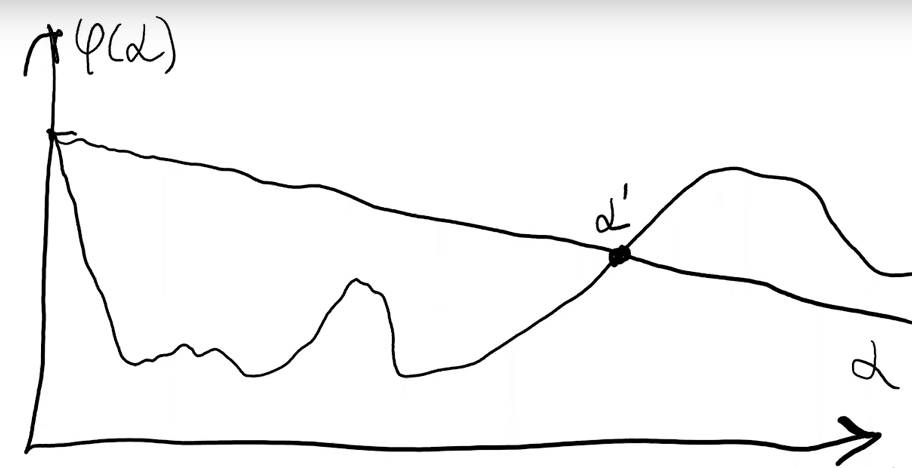
\includegraphics[scale=0.4]{img/methopt_volfe_conditions_proof}
\end{center}
    Заметим, что первое условие выполнятется всюду, где $\alpha < \alpha^\prime$.
    Почему где-то на этом интервале выполнится второе условие?
    
    \[f(x_k  + \alpha^\prime p_k) - f(x_k) = \alpha^\prime \triangledown f(p_k +\alpha^{\prime\prime} p_k) p_k, ~~~ \text{где } \alpha^{\prime\prime} ~\text{ --- некоторая неизвестная нам точка}. \]
    Тогда,
    \[ \triangledown f(x_k + \alpha^{\prime\prime} p_k) \cdot p_k = c_1 \triangledown f(x_k) \cdot p_k > c_2 \triangledown f (x_k) p_k. \]
    Таким образом, $\alpha^{\prime\prime}$ удовлетворяет второму условию Вольфе.
\end{proof}

Введем обозначение $\cos \Theta = \dfrac{-\triangledown f(c_k) \cdot p_k}{\| \triangledown f(x_k) \| \|p_k\}}$.

\begin{theorem}
    Если $p_k$~--- направление поиска, $\alpha_k$ удовлетворяет условиям Вольфе,
    $f$ огра\-ни\-че\-на и непрерывно дифференцируема и градиент функции $f$ является Липшица--непрерыным ($\| \triangledown f - \triangledown f(\overline{x}) \| \leqslant L \| x - \overline{x} \|$, ~$L > 0$). Тогда будет выполняться следующее соотношение 
    \[\sum_{k\geqslant 0} \cos^2 \Theta_k \| \triangledown f(x_k)\|^2 < +\infty. \]
\end{theorem}
\begin{remark}
    Если $\cos^2 > 0$, то последовательность градиентов должна стремится к 0.
\end{remark}
\begin{proof}
    \[\underbrace{\left( \triangledown f(x_{k + 1}) - \triangledown f(x_k) \right) \cdot p_k}_{\leqslant \alpha_k L \| p_k\| ^2} \geqslant (c_2 - 1) \cdot \triangledown f(x_k) \cdot p_k. \]
    Выразим $\alpha_k$:
    \[\alpha_k \geqslant \dfrac{c_2 - 1}{L} \cdot \dfrac{\triangledown f(x_k) \cdot p_k}{\| p_k \|^2}.\]
    Скомбинируем условие на $\alpha$ с первым условием:
    \[f(x_k) \leqslant f(x_k) - \underbrace{c_1 \dfrac{1 - c_2}{L} \cdot \dfrac{\left( \triangledown f(x_k) \cdot p_k \right)^2}{\|p_k \|^2} }_{-c \cos^2 \Theta \cdot \| \triangledown f(x_k) \| ^2, ~~c = \frac{c_1 (1 - c_2))}{L}}
    \implies
    f(x_{k+1}) \leqslant f(x_0) - c \sum_{j = 0}^k \cos^2 \Theta \| \triangledown f(x_j) \|^2.\]
    Так как фукция была огранчиена, то ряд ограничен и сходится.
\end{proof}

\subsection{Стахастический градентный спуск}
\begin{problem}[Линейная регрессия]
    Пусть у нас есть некоторые точки на плоскости. Мы хотим провести некоторую прямую, чтобы минимизировать сумму квадратов отклонений.

    \begin{center}
        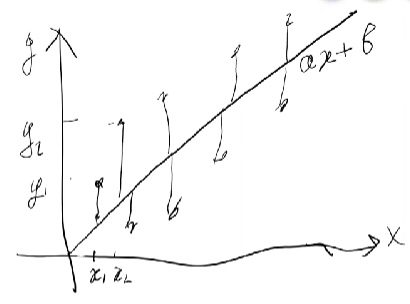
\includegraphics[scale=0.5]{img/linear_regression_problem}
    \end{center}

    Пусть есть функция $f(a, b) = \sum_{i=1}^n \left( a x_i + b - y_i \right)^2$. Хотим найти такие $a, b$, что $f$ принемает минимальное значние.

    Вообще, задачу можно решить аналитически.

    Но если обощить ее  на пространство более высокой размерности, аналитиечски решать будет сложно, численные методы лучше.

    Можно переформулировать задачу в матричном виде:
    \[Y = \begin{pmatrix}
        y_1\\ y_2\\ \dots\\ y_n 
    \end{pmatrix}, ~~~X = \begin{pmatrix}
        x_{1,1} & \dots & x_{1,n}\\
        \dots & \dots & \dots\\
        x_{n,1} & \dots & x_{n,n}.
    \end{pmatrix}, ~~~
    f = \| X \beta - Y \| ^2 \implies
    \beta = \left( X^T X \right) ^{-1} X ^T Y.\]

    Если размерность большая, это не сработает.
\end{problem}

\begin{definition}
    Пусть $f(x) = \sum\limits_j Q_j (x)$.

    Стахастический градиентный спуск заключается в выборе одного случайного слогаемого в сумме, вычислении градиента этого слогаемого и спуск по этому градиенту.
\end{definition}

\begin{itemize}
    \item[+] Один шаг очень дешевый.
    \item[-~] Результат от одного шага достаточно сомнительный,  поэтому говорить о сходимости данного метода не приходится.
    \item[-~] Найти точный минимум очнеь сложно.
\end{itemize}

У данного метода есть достаточно много модификаций.

Одна из наиболее популярных модификаций~--- \textbf{Mini Batch Gradient Descent}.
\subsubsection{Mini Batch Gradient Descent}
Мы можем проводить полный градиентный спуск, то есть считать граент по всем $n$ слогаемым (тяжело вычислять). Можем проводить стахастичесий градиентный спуск и считать градиен по одному слогаемому (получается не точно). А можем выбрать, например $10$ случайных слогаемых и посчитать по ним градиент.

В machine learning обыно выбирают не случайные слогаемые, а спрева перемешивают, а затем последовательно рассматривают первые $k$, вторые $k$ и т.д. слогаемых.
